\documentclass[a4paper,12pt]{article}
\usepackage{amsmath}
\usepackage{graphicx}
\usepackage{lipsum}
\usepackage{hyperref}
\hypersetup{
    colorlinks=true,       
    linkcolor=blue,        
    urlcolor=blue,        
}
\usepackage[T1]{fontenc}

\begin{document}
\title{5. Digital Filter Design and Analysis: Implementing
 FIR and IIR filters in Python.
 6. Adaptive Filtering: Applying adaptive filtering
 algorithms to noise reduction.}
\author{Daria Kręcichwost}
\date{\today}

\begin{titlepage}
    \centering
    \vspace*{2cm}
    
    \Huge
    REPORT
    
    \vspace{1cm}
    
    \Large
    Course: Analog and digital electronic circuits \\
    Teacher: Prof. Dr. Hab. Vasyl Martsenyuk
    
    \vfill
    
    \Large
    Lab No. 5 and 6\\
    Date: \today \\
    Topic: "Filtering" \\
    Variant: 8
    
    \vspace{1cm}
    
    \large
    Name: Daria Kręcichwost \\
    Computer Science (Second Degree) \\
    Part-time studies, Semester 1 \\
    Group: B
\end{titlepage}

\newpage
\maketitle

\section{Problem Statement}
The task is to design and implement three different types of filters to reduce noise in a noisy sinusoidal signal:
\begin{enumerate}
    \item Design a Finite Impulse Response (FIR) filter with the given coefficients \( b = [1, 0, 1] \).
    \item Design an Infinite Impulse Response (IIR) filter with the given coefficients \( b = [0.5, 0.5] \) and \( a = [1, -0.3] \).
    \item Implement an Adaptive Least Mean Squares (LMS) filter with a step size \( \mu = 0.05 \) and filter length \( M = 5 \).
\end{enumerate}

\section{Input Data}
The input signal for the task is a noisy sinusoidal signal. The sinusoidal signal has a frequency of 5 Hz and is sampled at a frequency of 1000 Hz. Gaussian noise is added to this sinusoidal signal to simulate a noisy signal.

\[
x(t) = \sin(2 \pi f t) + \text{Noise}
\]
where \( f = 5 \) Hz.

The desired signal is the clean sinusoidal signal without noise.

\section{Commands Used}
\subsection{Source Code}

The source code for the filter implementations is written in Python and uses the NumPy library for numerical computations and Matplotlib for plotting. Below is a summary of the code sections for the FIR, IIR, and LMS filters.
\item
\href{https://github.com/DariaKrecichwostQA/StudiaUBB/tree/main/Digital%20Signal%20Processing/Zad3}{{Link to remote repository on GitHub}}
\subsubsection{FIR Filter}

The FIR filter uses the coefficients \( b = [1, 0, 1] \) and convolves the input signal with the filter coefficients.

\begin{verbatim}
import numpy as np
import matplotlib.pyplot as plt

def fir_filter(x, b):
    M = len(b)
    y = np.zeros(len(x))
    for n in range(M, len(x)):
        y[n] = np.dot(b, x[n-M+1:n+1][::-1])
    return y
\end{verbatim}

\subsubsection{IIR Filter}

The IIR filter uses the coefficients \( b = [0.5, 0.5] \) and \( a = [1, -0.3] \). It applies both feedforward and feedback operations to calculate the output signal.

\begin{verbatim}
def iir_filter(x, b, a):
    M = len(b)  # Length of numerator coefficients (b)
    N = len(a)  # Length of denominator coefficients (a)
    y = np.zeros(len(x))  # Initialize output signal array

    for n in range(len(x)):
        x_slice = x[max(0, n-M+1):n+1]  # Input signal slice
        y[n] = np.dot(b[:len(x_slice)], x_slice[::-1])

        if n >= 1:
            y_slice = y[max(0, n-N+1):n]
            y[n] -= np.dot(a[1:], y_slice[::-1])

    return y
\end{verbatim}

\subsubsection{LMS Filter}

The LMS filter is an adaptive filter that adjusts its weights based on the error between the desired and actual output.

\begin{verbatim}
def lms_filter(x, d, mu, num_taps):
    n = len(x)
    w = np.zeros(num_taps)
    y = np.zeros(n)
    e = np.zeros(n)

    for i in range(num_taps, n):
        x_segment = x[i-num_taps:i][::-1]
        y[i] = np.dot(w, x_segment)
        e[i] = d[i] - y[i]
        w += mu * e[i] * x_segment
    
    return y, e, w
\end{verbatim}

\subsection{Screenshots}

\vfill
\begin{figure}[htbp]
\centering
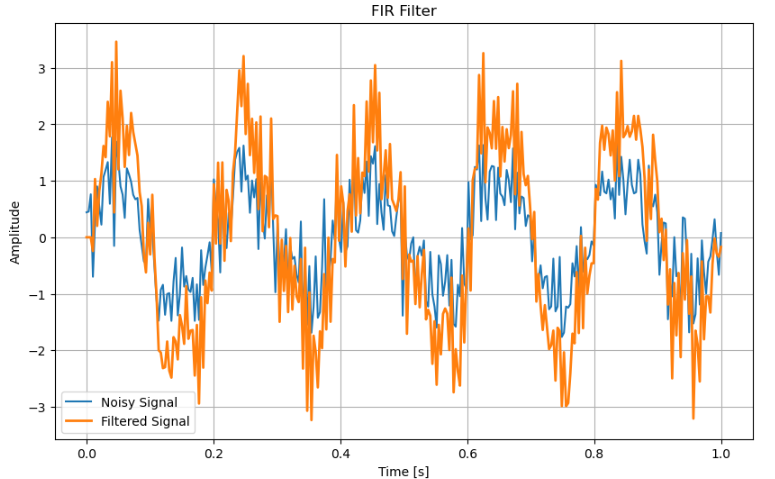
\includegraphics[width=\textwidth]{Zad 3/fir_filter_output.png} 
\caption{FIR Filter Response}
\label{fig:window_spectra_comparison}
\end{figure}

\begin{figure}[htbp]
\centering
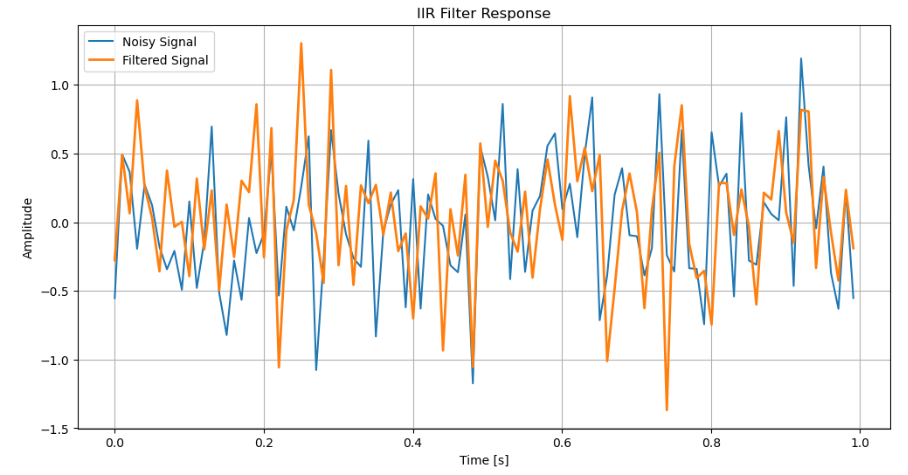
\includegraphics[width=\textwidth]{Zad 3/iir_filter_output.png} 
\caption{IIR Filter Response}
\label{fig:window_spectra_comparison}
\end{figure}

\begin{figure}[htbp]
\centering
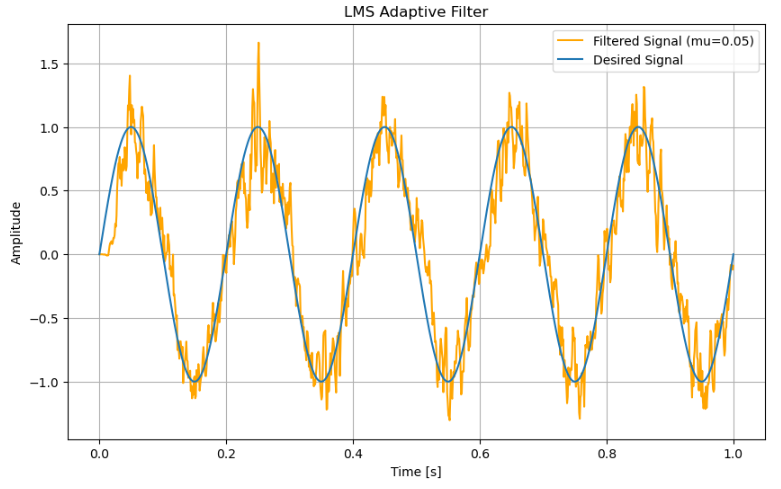
\includegraphics[width=\textwidth]{Zad 3/lms_filter_output.png} 
\caption{LMS Filter Response}
\label{fig:window_spectra_comparison}
\end{figure}

\section{Outcomes}
The results obtained from the FIR, IIR, and LMS filters are as follows:
\begin{enumerate}
    \item The FIR filter successfully reduces high-frequency noise, although some residual noise remains.
    \item The IIR filter provides a smoother output, especially for higher frequencies.
    \item The LMS adaptive filter is able to adjust dynamically to the noise, producing a clean signal by minimizing the error between the desired and actual signal.
\end{enumerate}
\newpage
\section{Conclusions}
\begin{enumerate}
    \item The FIR filter is effective for reducing noise but may not perform as well as the IIR and LMS filters in all cases.
    \item The IIR filter provides a more efficient solution for noise reduction with less residual noise compared to the FIR filter.
    \item The LMS adaptive filter performs the best in terms of adaptability, adjusting the filter parameters to minimize the error and providing the cleanest output signal.
\end{enumerate}

\end{document}
